\documentclass{article}
\usepackage[utf8]{inputenc}

\usepackage[
backend=biber,
style=alphabetic,
citestyle=authoryear
]{biblatex}
\usepackage{natbib}
\usepackage{graphicx}
\usepackage{amsmath}
\usepackage[utf8]{inputenc}
\usepackage{float} 
\usepackage{subfigure}
\usepackage{ragged2e}

\title{Digital Tools for Finance}
\author{Kun Zhang, Ziyun Ni, Ruixuan Zhou, Kevin Hardegger }
\date{15 December 2020}

\begin{document}

\maketitle

\section{Introduction}
There is a theory which states that if ever anyone discovers exactly what the Universe is for and why it is here, it will instantly disappear and be replaced by something even more bizarre and inexplicable.
There is another theory which states that this has already happened.


\section{Beta as risk measure}
According to the CAPM, the expected return of any stock is equal to the return on the riskless asset plus the market beta of this stock plus the market risk premium. Expressed mathematically, the CAPM is

\begin{equation}
    E[R_{i,t}]=R_{f,t}+\beta_{i}(E[R_{m,t}-R_{f,t}])
\end{equation}
where the security’s beta is given by


\begin{equation}
     \beta_{i}=\frac{Cov(R_{i,t},R_{m,t})}{Var(R_{m,t})} 
\end{equation}
The fundamental prediction of the CAMP theory is that there is a positive relation between market beta and expected stock returns, and the slope defining thsi relation represents the market risk premium. Thus, we would expect to find a positive cross-sectional relation between beta and future excess return.

\section{Evaluating beta-based portfolio}
First, we created time series for both datasets, daily betas and daily prices of all stocks that belonged to the SMI. Second, we used daily prices to estimate the daily returns for each stock. Then, for each period of the time series, we ranked the stocks included in the SMI based on their betas in the previous period and divided them into 5 portfolios based on the quintiles 20\%, 40\%, 60\% and 80\%. Subsequently, we continued this process until the last period of the time series. Finally, for each portfolio we calculated the average daily return and the average standard deviation of the daily returns. The table below summarizes the results:


\makeatletter\def\@captype{table}\makeatother
\centering
\resizebox{1\textwidth}{!}{%
\begin{tabular}{|l|c|c|c|c|c|}
\hline
\multicolumn{1}{|l|}{} & P1      & P2      & P3      & P4      & P5      \\ \hline
Mean daily return      & 0.027\% & 0.035\% & 0.041\% & 0.058\% & 0.039\% \\ \hline
Mean standard deviation           & 0.958\% & 1.268\% & 1.455\% & 1.620\% & 1.972\% \\ \hline
\end{tabular}%
}
\caption{Mean daily returns \& mean standard deviation of each beta-sorted portfolio}
\label{tab:my-table}

~\\
\begin{justify}
From above, we can clearly see that the mean standard deviation is low if a portfolio contains stocks with low beta and is high if a portfolio contains the stocks high beta. The magnitudes of the mean daily returns of portfolios 1 to 4 is consistent with the magnitudes of their mean standard deviation. The higher the average standard deviation respective the volatility, the higher the average daily return. One exception is the portfolio 5. It has the highest volatility but surprisingly not the highest mean return, which contradicts the Mean-Variance theory.
We first calculated cumulative returns for each portfolio and we then plotted them. The plot of the development of each portfolio’s cumulative returns is shown below
\begin{figure}[H]
\centering
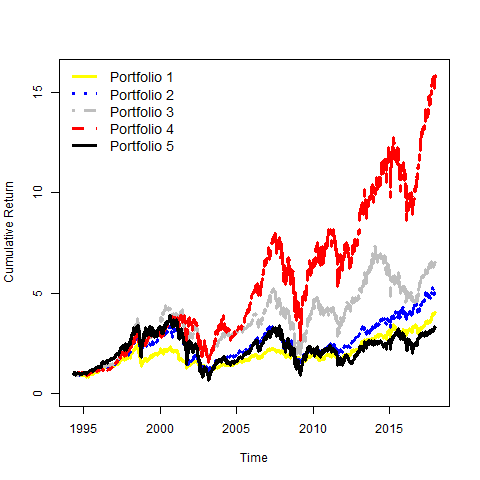
\includegraphics[width=1\textwidth,height=0.7\textwidth]{Cumulative Returns}
\caption{Cumulative Returns}
\label{fig:Cumulative Returns}
\end{figure}



To ensure that the daily beta of each portfolios are correctly ordered, we also draw a line 
\begin{figure}[H]
\centering
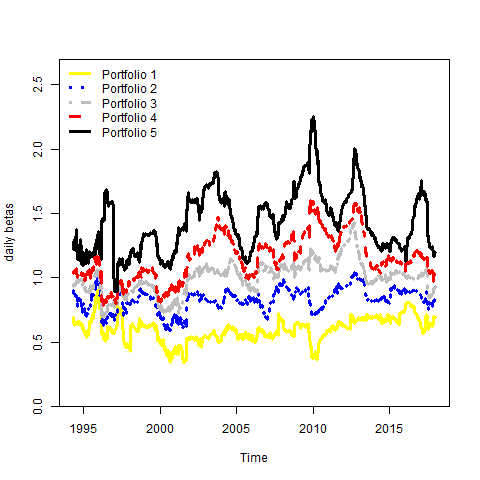
\includegraphics[width=1\textwidth,height=0.7\textwidth]{daily betas}
\caption{daily betas}
\label{fig:daily betas}
\end{figure}
From the above chart, we can clearly see that the cumulative return of portfolio 4 is the highest, although the beta of the stocks contained in portfolio 4 are only the second highest. The magnitudes of the cumulative returns of portfolios 1 to 4 is also consistent with the magnitudes of the betas of stocks contained in each portfolio. But surprisingly, although Portfolio 5 contains stocks with the highest beta, his returns are the lowest, which contradicts the CAPM theory that predicts a positive relation between beta and expected returns.
The risk of a stock can be measured by its standard deviation. However, it can be reduced by diversification effect respective by holding other stocks in a portfolio. This means that the right way to measure the risk of a stock is not by its standard deviation but rather by its covariance with the market portfolio. Thus, the CAPM beta should be a more appropriate risk measure.  But our empirical result above fails to produce supporting evidence, since portfolio 5 should have the highest cumulative return among those beta-sorted portfolios according to the CAPM theory.


\section{Conclusion}
``I always thought something was fundamentally wrong with the universe'' \citep{adams1995hitchhiker}
\end{justify}


\end{document}